\textbf{Цель работы:} изучение вольт-амперной характеристики тлеющего разряда; изучение свойств плазмы методом зондовых характеристик.\\\indent
\textbf{Оборудование:} стеклянная газоразряданя трубка, наполненная неоном, высоковольтный источник питания, источник питания постоянного тока, делитель напряжения, резистор, потенциометр, амперметры, вольтметры, переключатели.

\section*{Теоретические сведения}
\begin{wrapfigure}{r}{0.3\linewidth}
    \centering
    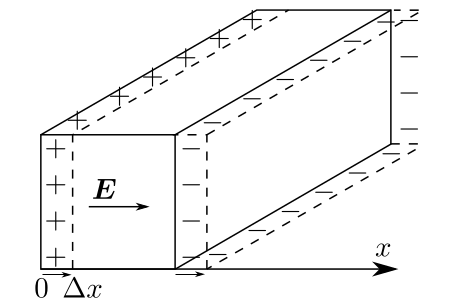
\includegraphics[width=6cm]{images/flactuation.png}
    \caption{Плазменные колебания}
\end{wrapfigure}
Если газ продолжать нагревать, то сначала молекулы диссоциируют на атомы, а затем и
атомы распадаются на электроны и ионы, так что газ становится ионизованным, представляя собой смесь из свободных электронов и ионов,а также нейтральных частиц.
Газ с достаточно большой степенью ионизации называют плазмой.\\\indent
Рассмотрим простейший вид \textbf{плазменных колебаний}. Ионы будем считать одноразрядными т.е $n_i = n_e$. Выделим в нейтрильной плазме некоторый объем (рис.1). Пусть все электроны сместились на расстояние $x$ относительно ионов (ионы как существенно тяжелые частицы можно считать неподвижными). Тогда на боковых гранях возникнут поверхностные заряды с плотностю $\sigma = \pm n_e e \Delta x \text{  }\Rightarrow E = 4 \pi n_e e \Delta x \text{  }\Rightarrow \text{  } \ddot{x} = -\frac{eE}{m} = -\frac{4\pi n_e e^2}{m}x \text{  } \Rightarrow \text{  } \omega = \sqrt{\frac{4\pi n_e e^2}{m}}$ - плазменная (ленгмюровская) частота коллективных колебаний электронов.\\
\indent Определим амплитуду колебаний в случае, когда колебания возбуждены за счет тепловой энергии. Средняя скорость теплового движения $\bar v_e = \sqrt{\frac{kT_e}{m_e}}$. Амплитуду колебаний оценим как смещение с этой скоростю за характерное вермя плазменных колебаний $1 / \omega$ 
\begin{equation}
    r_D \approx \frac{\bar v_e}{\omega} = \sqrt{\frac{kT_e}{4\pi n_e e^2}}
\end{equation}
$r_D$ - \textbf{дебаевский радиус}. \textbf{Идеальной плазмой} называется ионизованный газ, дебаевский радиус которого существенно меньше характерного размера области, занимаемой этим газом.\\\indent
Простым методом исследования свойств плазмы является измерение электрических потенциалов с помощью \textbf{зонов} - небольших проводников, вводимых в плазму. При внесении в плазму он сталкивается с заряженными частицами. И т.к скорости электронов существенно превышает скорости ионов, то проводник зарядится отрицательно $-U_f$. Рассмотрим измерения с помощью \textbf{двойного зонда} - система, состоящая из двух одинаковых зондов, расположенных на небольшом расстоянии друг от друга. Между зондами создаётся разность потенциалов 𝑈 , которая по величине
много меньше плавающего потенциала $|U| \ll |U_f|$. При этом оба зонда
имеют относительно плазмы близкий к плавающему отрицательный по­
тенциал.Рассчитаем величину тока, проходящего через двойной зонд вблизи
точки $I = 0$.
\begin{equation}
    I = I_{iн}\th\frac{e U}{2kT_e}
\end{equation}

\section*{Экспериментальные данные и установка}
\indent Стеклянная газоразрядная трубка имеет холодный полый катод, три анода и геттерный узел — стеклянный баллон, на внутреннюю поверхность которого напылена газопоглощающая плёнка (геттер).
\noindent Катод и один из анодов (I или II) с помощью переключателя П1 к регулируемому высоковольтному источнику питания (ВИП) с выходным напряжением до нескольких киловольт. При подключении к ВИП анода-I между ним и катодом возникает газовый разряд.
Ток разряда измеряется миллиамперметром A1, а падение напряжения на разрядной трубкевольтметром V1. При подключении к ВИП анода-II разряд возникает в пространстве
между катодом и анодом-II, где находится двойной зонд, используемый для диагностики плазмы положительного столба.
Зонды изготовлены
из молибденовой проволоки диаметром $d = 2$  мм и имеют длину $l = 5.2$ мм. Они подключены к источнику питания через потенциометр R. Переключатель П2 позволяет изменять полярность напряжения на зондах.
Для измерения зондового тока используется микроамперметр A2. 
\begin{figure}[h!]
    \begin{subfigure}{0.5\linewidth}
        \centering
        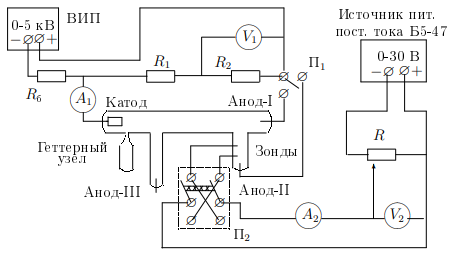
\includegraphics[width=9.5cm]{setup.png}
        \caption*{Cхема экспериментальнoй установки}
    \end{subfigure}
    \hfill
    \begin{subfigure}{0.5\linewidth}
        \centering
        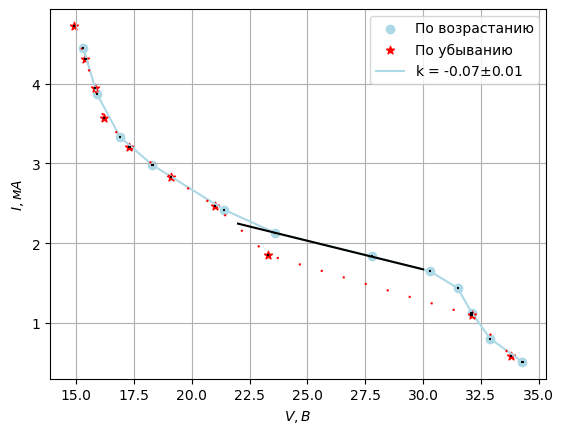
\includegraphics[width=9.5cm]{images/plot1.png}
        \caption*{ВАХ разряда при убывании и нарастании тока}
    \end{subfigure}
\end{figure}


\subsection*{\normalsize{Вольт-ампераня характеристика разряда}}
\normalsize{Определим напряжение зажигания разряда $U_{\text{разр}} = 200$ В. Из графика находим $R_{\text{диф}}^{\text{max}} = \frac{dU}{dI} = (13.98 \pm 0.05)\cdot 10^{3}$ Ом}
\begin{table}[h!]
    \centering
    \begin{tabular}{|c|c|c|c|c|c|c|c|c|c|c|}
        \hline
        (нарастание)$I$, мА & 0.52& 0.80& 1.13& 1.439& 1.84& 2.42& 2.98& 3.33& 3.87& 4.45\\\hline
        (нарастание)$U$, В & 34.3& 32.9& 32.1& 31.5& 27.8& 21.4& 18.3& 16.9& 15.9& 15.3\\\hline

        (убывание)$I$, мА & 4.721& 4.31& 3.939& 3.570& 3.203& 2.827& 2.469& 1.852& 1.100& 0.594\\\hline
        (убывание)$U$, В & 14.9& 15.4& 15.8& 16.2& 17.3& 19.1& 21.0& 23.3& 32.1& 33.8\\\hline
    \end{tabular}
    \caption{ВАХ разряда при нарастании и убывании тока}
\end{table}

\newpage
\subsection*{\normalsize{Зондовые характеристики}}
Cнимем вольт-амперную характеристику двойного зонда для различных значений разрядного тока $I_{\text{р}}$. По полученным графикам определим температуру электронов по формуле:
\begin{equation}
    kT_e = \frac{1}{2}\frac{eI_{\text{iн}}}{\frac{dI}{dU}\vline_{U=0}}
\end{equation}
Определим так же ионный ток насыщения $I_{\text{iн}}$ и концентрацию $n_e = n_i = n$ через этот ток:
\begin{equation}
    I_{iн} = 0.4n_ieS\sqrt{\frac{2kT_e}{m_i}}
\end{equation}
Рссчитаем плазменную частоту колебаний $\omega$, электронную поляризационную длину $r_{D_e}$ и число ионов $N_D$ в дебаевской сфере по формулам соответсвенно:

\begin{align}
\omega &= \sqrt{\frac{4\pi n_e e^2}{m_e}} = 5.6\cdot 10^{4}\sqrt{n_e}\\
r_{D_e} &= \sqrt{\frac{kT_e}{4\pi n_e e^2}}\\
N_D &= \frac{4}{3}\pi {r_D}^3 n_i\\
r_D &\approx \frac{\bar v_e}{\omega} = \sqrt{\frac{kT_e}{4\pi n_e e^2}}
\end{align}

\begin{table}[h!]
    \centering
    \begin{tabular}{|c|c|c|c|c|}
        \hline
        $I_{\text{р}}$, мА & 5 \pm 0.02 & 4 \pm 0.02& 3 \pm 0.02& 1.5 \pm 0.02\\\hline
        $\Delta U$, В & 11.5 \pm 0.5 & 10.3 \pm 0.3 &  8.1 \pm 0.4 & 7\pm 0.5 \\\hline 
        $I_{\text{iн}}$, мкА & 79.8 \pm 9.3 & 70\pm 8& 44.5 \pm 6.5 & 21.4 \pm 3.7\\\hline 
        $T_e, K\cdot 10^3$& 68 \pm 8 & 60\pm 7 & 47\pm 7&18\pm 3\\\hline
        $n$, $\text{м}^{-3}\cdot 10^{16}$ & 5.3\pm 0.6 & 5 \pm 0.6& 3.6\pm 0.5 & 2.7\pm 0.5\\\hline
        $\omega$, рад/с $\cdot 10^4$& 13.6\pm 1.6& 13.2\pm1.5 & 11.1\pm 1.7& 9.7\pm 1.8\\\hline
        $r_{D_e}$, мкм &  60.6\pm7.9& 62.2\pm7.5 & 69.8\pm11.3 &91.9\pm18.3 \\\hline
        $r_{D}$, мкм &  4.32\pm0.60& 5.13\pm0.76& 5.68\pm0.97 & 7.96\pm1.62 \\\hline
        $N_D$ & 26.3 \pm 3.6 & 29.6\pm 4.4&  34.5\pm5.9 & 48.4\pm9.8\\\hline
        $\alpha, 10^(-7)$ & 12.06\pm0.06&8.54\pm0.05 & 7.00\pm0.04 & 3.56\pm0.02 \\\hline
    \end{tabular}
    \caption{Данные найденные по ВАХ зонда для различных значений тока разряда}
\end{table}


\newpage
\begin{table}[h!]
    \centering
    \begin{tabular}{|c|c|c|c|c|c|c|c|c|c|c|c|c|c|}
        \hline
        \multirow{2}{*}{$I_{\text{р}} = 5$ мА} & $I$, мА & 82.5&85.9&84.7&81.5&74.6&62.4&50.6&36.5&19.9&-24.4&-42.5&-51.9\\
        &$U$, В & 25.01&  22.03&  19.  &  16.04&  13.03&  10.04&   8.01&   6.02& 4.03&  -2.02&  -4.08&  -6.01\\\hline
        \multirow{2}{*}{$I_{\text{р}} = 4$ мА} & $I$, мА & 70.6&  70.3&  68.5&  65.7&  60.6&  51.1&  42.3&  30.5&  17.1&
       -23.5& -38.9& -51.5\\
       &$U$, В & 25.03& 22.08& 19.04& 16.  & 13.04& 10.02&  8.06&  6.07&  4.01&
       -2.04& -4.06& -6.06\\\hline
       \multirow{2}{*}{$I_{\text{р}} = 3$ мА} & $I$, мА & 52.6 &  50.9 &  49.17&  47.2 &  44.  &  38.1 &  32.02&  23.5 &
        13.5 & -20.3 & -31.5 & -41.0\\
       &$U$, В & 25.03& 22.04& 19.03& 16.06& 13.04& 10.03&  8.07&  6.  &  4.03&
       -2.03& -4.08& -6.08\\\hline
       \multirow{2}{*}{$I_{\text{р}} = 1.5$ мА} & $I$, мА & 24.6&  23.8&  23. &  22.2&  21.1&  18.8&  16.1&  12.2&   7.1&
       -12.3& -17.9& -22.7\\
       &$U$, В & 25.  & 22.09& 19.06& 16.03& 13.08& 10.06&  8.05&  6.04&  4.09&
       -2.17& -4.06& -6.02\\\hline
    \end{tabular}
    \caption{Данные ВАХ двойного зонда при различных токах разряда}
\end{table}
\begin{figure}[h!]
    \centering
    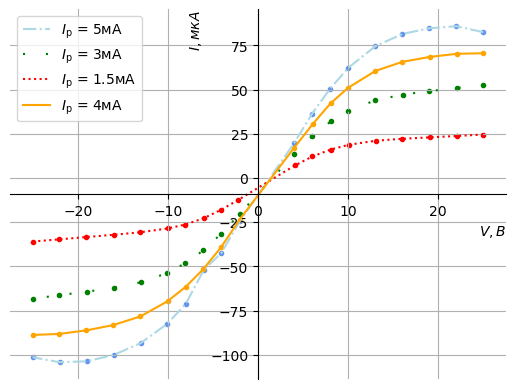
\includegraphics[width=15cm]{images/plot2.png}
    \caption{Сравнение ВАХ двойного зонда при различных токах разряда}
\end{figure}

\newpage

\begin{figure}[h!]
    \begin{subfigure}{0.5\linewidth}
        \centering
        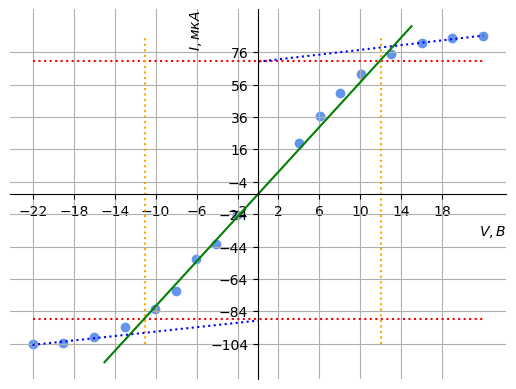
\includegraphics[width=10cm]{images/plotI_5.png}
        \caption{При $I_{\text{р}}$ = 5 мА}
    \end{subfigure}
    \hfill
    \begin{subfigure}{0.5\linewidth}
        \centering
        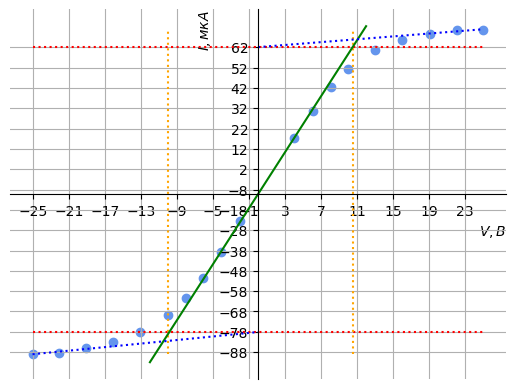
\includegraphics[width=10cm]{images/plotI_4.png}
        \caption{При $I_{\text{р}}$ = 4 мА}
    \end{subfigure}
    \vfill
    \begin{subfigure}{0.5\linewidth}
        \centering
        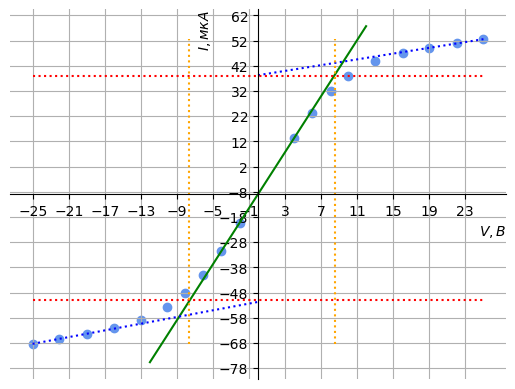
\includegraphics[width=10cm]{images/plotI_3.png}
        \caption{При $I_{\text{р}}$ = 3 мА}
    \end{subfigure}
    \hfill
    \begin{subfigure}{0.5\linewidth}
        \centering
        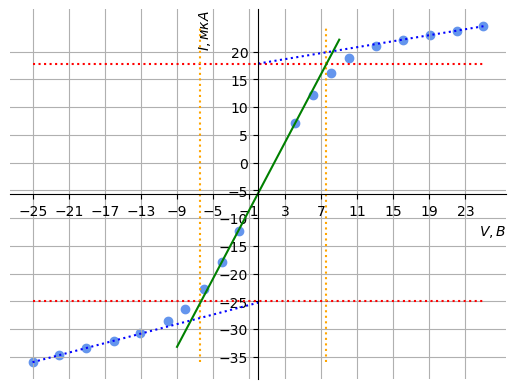
\includegraphics[width=10cm]{images/plotI_1.5.png}
        \caption{При $I_{\text{р}}$ = 1.5 мА}
    \end{subfigure}
    \caption{ВАХ двойного зонда при различных значениях тока разряда $I_{\text{р}}$}
\end{figure}


